\documentclass[tikz,border=4pt]{standalone}
\usetikzlibrary{positioning,arrows.meta,fit,backgrounds,calc}

% Color definitions (Okabe-Ito / Color Universal Design compliant)
\definecolor{cEnergy}{HTML}{D55E00} % Vermillion for energy
\definecolor{cInfo}{HTML}{0072B2}   % Blue for information

\tikzset{
  box/.style={
    draw=black!85,
    rounded corners=2pt,
    align=center,
    font=\scriptsize,
    minimum height=7mm,
    inner sep=3.5pt,
    fill=white,
    line width=0.6pt
  },
  hub/.style={
    box,
    fill=gray!12,
    draw=black,
    line width=1.1pt,
    font=\scriptsize\bfseries
  },
  groupbox/.style={
    draw=gray!50,
    dashed,
    rounded corners=3.5pt,
    fill=gray!4,
    inner sep=5pt,
    line width=0.6pt
  },
  energy/.style={
    -{Stealth[length=1.8mm,width=1.3mm]},
    cEnergy,
    line width=1.1pt
  },
  energyBi/.style={
    {Stealth[length=1.8mm,width=1.3mm]}-{Stealth[length=1.8mm,width=1.3mm]},
    cEnergy,
    line width=1.1pt
  },
  energyLine/.style={
    cEnergy,
    line width=1.1pt
  },
  info/.style={
    -{Stealth[length=1.6mm,width=1.2mm]},
    cInfo,
    line width=0.9pt,
    dashed
  },
  infoBi/.style={
    {Stealth[length=1.6mm,width=1.2mm]}-{Stealth[length=1.6mm,width=1.2mm]},
    cInfo,
    line width=0.9pt,
    dashed
  },
  grouplabel/.style={
    font=\scriptsize\bfseries,
    text=black!75
  }
}

\begin{document}
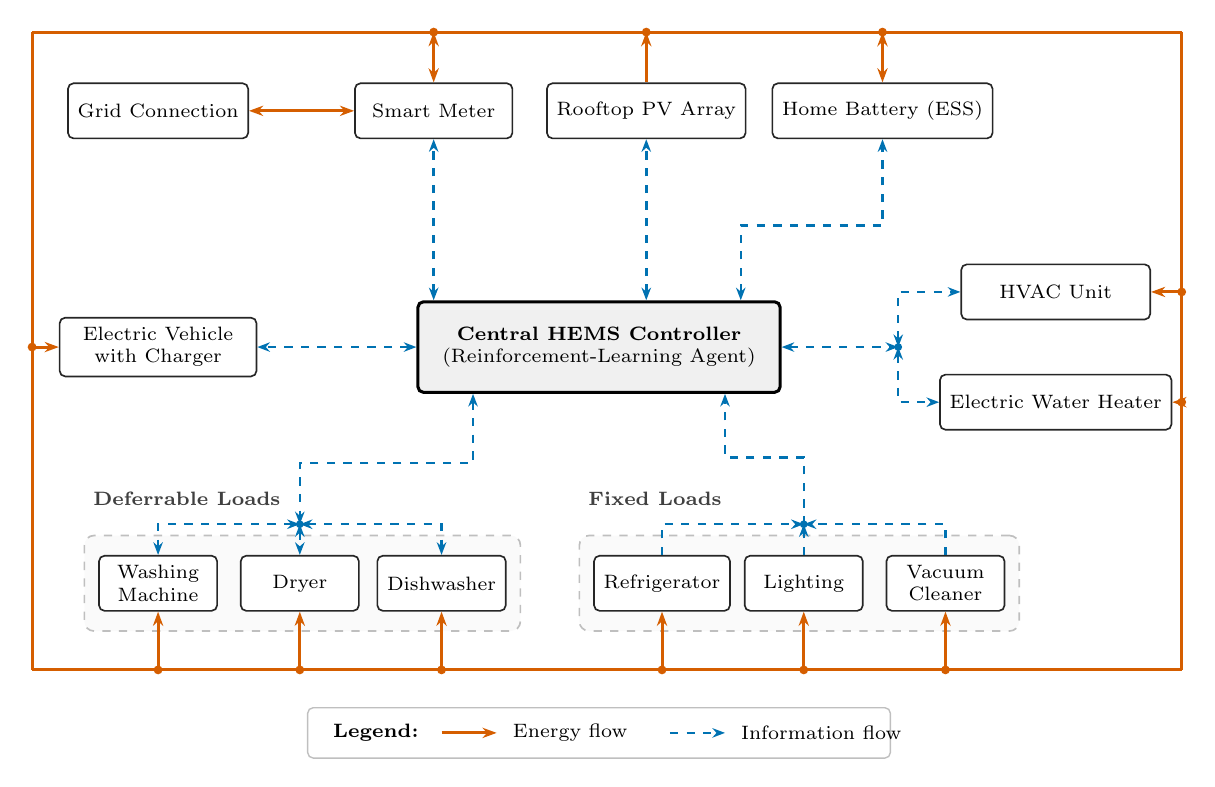
\begin{tikzpicture}

  % ========================================================
  % 1. NODES
  % ========================================================

  % Top row: External / Generation / Storage
  \node[box, minimum width=2.2cm] (grid)  at (-5.6, 3.4) {Grid Connection};
  \node[box, minimum width=2.0cm] (meter) at (-2.1, 3.4) {Smart Meter};
  \node[box, minimum width=2.4cm] (pv)    at ( 0.6, 3.4) {Rooftop PV Array};
  \node[box, minimum width=2.6cm] (ess)   at ( 3.6, 3.4) {Home Battery (ESS)};

  % Middle row: EV, Central Controller, HVAC, Water Heater
  \node[box, minimum width=2.5cm] (ev)   at (-5.6, 0.4) {Electric Vehicle\\with Charger};
  \node[hub, minimum width=4.6cm, minimum height=1.15cm] (ctl) at (0.0, 0.4) {
    Central HEMS Controller\\
    {\normalfont\scriptsize(Reinforcement-Learning Agent)}
  };
  \node[box, minimum width=2.4cm] (hvac) at ( 5.8, 1.1) {HVAC Unit};
  \node[box, minimum width=2.4cm] (ewh)  at ( 5.8, -0.3) {Electric Water Heater};

  % Bottom row: Deferrable Loads
  \node[box, minimum width=1.5cm] (wash)  at (-5.6, -2.6) {Washing\\Machine};
  \node[box, minimum width=1.5cm] (dryer) at (-3.8, -2.6) {Dryer};
  \node[box, minimum width=1.5cm] (dish)  at (-2.0, -2.6) {Dishwasher};

  % Bottom row: Fixed Loads
  \node[box, minimum width=1.5cm] (fridge) at ( 0.8, -2.6) {Refrigerator};
  \node[box, minimum width=1.5cm] (light)  at ( 2.6, -2.6) {Lighting};
  \node[box, minimum width=1.5cm] (vac)    at ( 4.4, -2.6) {Vacuum\\Cleaner};

  % Group bounding boxes (on background layer)
  \begin{scope}[on background layer]
    \node[groupbox, fit=(wash) (dryer) (dish), inner ysep=7pt, inner xsep=5pt] (deferrable_group) {};
    \node[groupbox, fit=(fridge) (light) (vac), inner ysep=7pt, inner xsep=5pt] (fixed_group) {};
  \end{scope}

  % Group labels (above group boxes, positioned to avoid crossing any line)
  \node[grouplabel, anchor=south west] at ([yshift=7pt] deferrable_group.north west) {Deferrable Loads};
  \node[grouplabel, anchor=south west] at ([yshift=7pt] fixed_group.north west) {Fixed Loads};

  % ========================================================
  % 2. ENERGY FLOWS (solid vermillion, outer distribution)
  % ========================================================

  % Direct grid connection to smart meter
  \draw[energyBi] (grid.east) -- (meter.west);

  % Outer perimeter coordinates
  \coordinate (busTL) at (-7.2, 4.4);
  \coordinate (busTR) at ( 7.4, 4.4);
  \coordinate (busBL) at (-7.2, -3.7);
  \coordinate (busBR) at ( 7.4, -3.7);

  % Top bus segment
  \draw[energyLine] (busTL) -- (busTR);
  \draw[energyBi] (meter.north) -- (meter.north |- busTL);
  \draw[energy]   (pv.north)    -- (pv.north |- busTL);
  \draw[energyBi] (ess.north)   -- (ess.north |- busTL);

  % Tap dots on top bus
  \fill[cEnergy] (meter.north |- busTL) circle (1.6pt);
  \fill[cEnergy] (pv.north |- busTL)    circle (1.6pt);
  \fill[cEnergy] (ess.north |- busTL)   circle (1.6pt);

  % Left bus segment (feeding EV)
  \draw[energyLine] (busTL) -- (busBL);
  \draw[energy] (-7.2, 0.4) -- (ev.west);
  \fill[cEnergy] (-7.2, 0.4) circle (1.6pt);

  % Right bus segment (feeding HVAC and Water Heater)
  \draw[energyLine] (busTR) -- (busBR);
  \draw[energy] (7.4, 1.1)  -- (hvac.east);
  \draw[energy] (7.4, -0.3) -- (ewh.east);
  \fill[cEnergy] (7.4, 1.1)  circle (1.6pt);
  \fill[cEnergy] (7.4, -0.3) circle (1.6pt);

  % Bottom bus segment (feeding appliances from below)
  \draw[energyLine] (busBL) -- (busBR);
  \draw[energy] (wash.south |- busBL)   -- (wash.south);
  \draw[energy] (dryer.south |- busBL)  -- (dryer.south);
  \draw[energy] (dish.south |- busBL)   -- (dish.south);
  \draw[energy] (fridge.south |- busBR) -- (fridge.south);
  \draw[energy] (light.south |- busBR)  -- (light.south);
  \draw[energy] (vac.south |- busBR)    -- (vac.south);

  % Tap dots on bottom bus
  \fill[cEnergy] (wash.south |- busBL)   circle (1.6pt);
  \fill[cEnergy] (dryer.south |- busBL)  circle (1.6pt);
  \fill[cEnergy] (dish.south |- busBL)   circle (1.6pt);
  \fill[cEnergy] (fridge.south |- busBR) circle (1.6pt);
  \fill[cEnergy] (light.south |- busBR)  circle (1.6pt);
  \fill[cEnergy] (vac.south |- busBR)    circle (1.6pt);

  % ========================================================
  % 3. INFORMATION FLOWS (dashed blue, central management)
  % ========================================================

  % Upward connections from HEMS Controller
  % Smart Meter: grid tariff signals & exchange telemetry
  \draw[infoBi] (ctl.north -| meter.south) -- (meter.south);

  % Rooftop PV: generation telemetry / curtailment
  \draw[infoBi] (ctl.north -| pv.south) -- (pv.south);

  % Home Battery (ESS): SoC sensing & charge/discharge dispatch
  \draw[infoBi] (ctl.north -| 1.8, 0) -- ++(0, 0.95) -| (ess.south);

  % Horizontal connection to EV
  \draw[infoBi] (ctl.west) -- (ev.east);

  % Horizontal/orthogonal connections to HVAC and Water Heater
  \coordinate (infoBranchThermal) at (3.8, 0.4);
  \draw[infoBi] (ctl.east) -- (infoBranchThermal);
  \draw[infoBi] (infoBranchThermal) |- (hvac.west);
  \draw[infoBi] (infoBranchThermal) |- (ewh.west);
  \fill[cInfo]  (infoBranchThermal) circle (1.4pt);

  % Downward connections to Deferrable Loads (scheduling / dispatch)
  % Trunk enters group area at x = -3.8 (well to right of "Deferrable Loads" label)
  \coordinate (infoBranchDef) at (-3.8, -1.85);
  \draw[infoBi] (ctl.south -| -1.6, 0) -- ++(0, -0.875) -| (infoBranchDef);
  \draw[infoBi] (infoBranchDef) -| (wash.north);
  \draw[infoBi] (infoBranchDef) -- (dryer.north);
  \draw[infoBi] (infoBranchDef) -| (dish.north);
  \fill[cInfo]  (infoBranchDef) circle (1.4pt);

  % Downward connections to Fixed Loads (power monitoring)
  % Trunk enters group area at x = 2.6 (well to right of "Fixed Loads" label)
  \coordinate (infoBranchFix) at (2.6, -1.85);
  \draw[info]   (infoBranchFix) -- ++(0, 0.85) -| (ctl.south -| 1.6, 0);
  \draw[info]   (fridge.north) |- (infoBranchFix);
  \draw[info]   (light.north)  -- (infoBranchFix);
  \draw[info]   (vac.north)    |- (infoBranchFix);
  \fill[cInfo]  (infoBranchFix) circle (1.4pt);

  % ========================================================
  % 4. LEGEND
  % ========================================================
  \begin{scope}[shift={(0.0, -4.5)}]
    \draw[draw=gray!50, rounded corners=2pt, fill=white, line width=0.5pt] (-3.7, -0.32) rectangle (3.7, 0.32);
    \node[font=\scriptsize\bfseries, anchor=west] at (-3.5, 0) {Legend:};
    \draw[energy, line width=1.1pt] (-2.0, 0) -- (-1.3, 0) node[right=2pt, font=\scriptsize, text=black] {Energy flow};
    \draw[info, line width=0.9pt]   (0.9, 0)  -- ( 1.6, 0) node[right=2pt, font=\scriptsize, text=black] {Information flow};
  \end{scope}

\end{tikzpicture}
\end{document}
